\documentclass[tikz,border=5pt]{standalone}
\usepackage{tikz}
\begin{document}
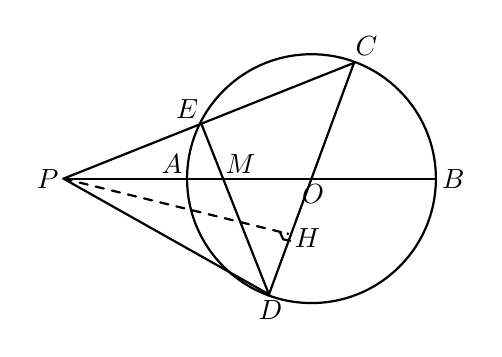
\begin{tikzpicture}[line cap=round, line join=round]

% 圆
\draw[thick] (3.80,-2.13) circle (1.58);

% 点坐标（单位 cm，y 轴取负以匹配原图方向）
\coordinate (P) at (0.65,-2.13);
\coordinate (A) at (2.22,-2.13);
\coordinate (B) at (5.38,-2.13);
\coordinate (O) at (3.80,-2.13);
\coordinate (M) at (2.67,-2.13);
\coordinate (C) at (4.34,-0.66);
\coordinate (E) at (2.40,-1.43);
\coordinate (D) at (3.26,-3.60);
\coordinate (H) at (3.50,-2.83);

% 直线
\draw[thick] (P) -- (B);      % 直径 AB 所在直线（延伸至 P）
\draw[thick] (P) -- (C);      % P-E-C
\draw[thick] (P) -- (D);      % 切线 PD
\draw[thick] (C) -- (D);      % 经过 O 的弦 CD
\draw[thick] (E) -- (D);      % 经过 M 的弦 ED
\draw[dashed, thick] (P) -- (H);

% 直角标记
\draw[thick] (3.40,-2.81) -- (3.44,-2.90) -- (3.53,-2.92);

% 点
\fill (C) circle (0.02);
\fill (E) circle (0.02);
\fill (D) circle (0.02);
\fill (H) circle (0.02);
\fill (M) circle (0.02);
\fill (O) circle (0.02);

% 标签（交换 H 与 M 的标签）
\node at (4.50,-0.45) {$C$};
\node at (2.22,-1.25) {$E$};
\node at (2.03,-1.95) {$A$};
\node at (2.90,-1.95) {$M$};   % 原 H 所在点，现标 M
\node at (3.75,-2.88) {$H$};   % 原 M 所在点，现标 H
\node at (3.82,-2.32) {$O$};
\node at (5.60,-2.13) {$B$};
\node at (0.45,-2.13) {$P$};
\node at (3.28,-3.80) {$D$};

\end{tikzpicture}
\end{document}
